\section{Introduction}
\label{s-intro}
Since its inception in 2008 \cite{bitcoin}, the blockchain technology has gained widespread attention as a transformative technology that can revolutionize many industries \cite{deloitte}. Blockchain based digital currencies such as Bitcoin \cite{bitcoin} and Ether \cite{Wood2014EthereumAS} are already being considered viable alternatives to existing currencies in trade and commerce for their security and ease of transfer. Blockchain smart contracts \cite{FM548} \cite{Wood2014EthereumAS}, on the other hand, have spawned innovative applications in many business and financial sectors due to their capacity of encoding the rules of interaction and ensuring their enforcement.

Central to the appeal of blockchain technology is its maintenance of a distributed ledger of transactions --  called the blockchain -- in a peer-to-peer network of autonomous and anonymous entities. In a blockchain network, all entities are even and none of them is trusted; still, the security and integrity of the transaction ledger can be guaranteed. This feat is achieved by a complete replication of information in all network participants where each participant validates and executes all transactions. As long as the majority of the network participants are honest, the outcome of the transactions, i.e., the state of the blockchain ledger can be trusted \cite{10.1007/978-3-319-56614-6_22}.

The blockchain technology's decentralization of trust through information and processing replication in a scalable peer-to-peer network is leading innovations and renovations in many application domains where trust and information security are key concerns. However, problem in one area in particular appears to be a major obstacle for blockchain based application adoption. This is the problem of document storage. 

The blockchain technology is inherently unsuitable for storing bulky information such as files and media contents due to the networking and storage cost associated with their management. Peculiarities of blockchain ledger maintenance such as \textit{blockchain reorg} \cite{reorg} further complicates the situation by making direct integration of existing trusted storage solutions with a blockchain network difficult. Finally, the continual preservation and integrity insurance requirement for trustworthy document storage is often in conflict with the incentive for blockchain transaction ledger maintenance that rewards participants for extending the ledger of transactions only and they can join or leave the network at any time.      

Nevertheless, there are some blockchain based or blockchain inspired storage technologies such as Ethereum Swarm \cite{swarm}, Filecoin \cite{filecoin}, Storj \cite{Wilkinson14storja}, and IPFS \cite{ipfs} already available for users. These solutions break down a user's file into a series or hierarchy of data chunks then distribute the chunks to the peer-to-peer network. On a broad level, some of these storage solutions are like traditional distributed hash tables \cite{Maymounkov:2002:KPI:646334.687801} \cite{10.1007/978-3-540-45172-3_4}. Some others are like peer-to-peer file sharing services such as the popular Bittorrent \cite{Pouwelse:2005:BPF:2138958.2138984}. These solutions apply some Bitcoin-like incentive mechanisms on top of these base technologies to motivate the network participants to retain and serve data chunks upon users' request.  

The motivation for these solutions is that they protect the users from vendor locked-in and they offer an overall larger storage capacity compared to existing storage alternatives. However, blockchain based solutions have the common problem that the owner (or user) has to take the responsibility of ensuring persistence and integrity of his/her data in the blockchain by retaining document metadata and issuing periodic audits. Furthermore, despite the combined storage capacity being huge, the download bandwidth can be significantly low as the network peers may be running commodity hardware behind low-speed network connections. In addition, designing incentive mechanisms for long-term persistent of documents in a mining based blockchain network is difficult 

Legacy databases of existing applications are also an obstacle for the applications' migration to the blockchain domain. Data stored in proprietary data centers are often confidential that a typical administrator may not be comfortable to put in the hands of anonymous blockchain participants. Further, when existing cloud storage providers \cite{Murty:2008:PAW:1407893} \cite{googleCloud} have already solved the storage capacity, scalability, and cost-effectiveness problems for the clients; there is little motivation for moving data into a blockchain storage.     

We believe to steer blockchain application innovations, blockchain technology should be supportive of existing storage solutions instead of being their competitor. In other words, the goal should be integrating existing storage technologies with blockchain -- not toppling them. A collaboration of technologies can bring the best of the both worlds. The blockchain technology can ensure integrity of external documents and control access to them according to the transparent governance of blockchain smart contracts and leave the actual storage, delivery, and capacity scaling to a matured storage technology. Here the blockchain technology is ideally suited for its part because information corruption in a blockchain network is very difficult and access rules written in the smart contracts are self-enforcing if integrated properly.

In our scheme, location, signature, access control configuration, upload/download fees and so on metadata information about a document is stored in some blockchain smart contract, called the {\it document bearer contract}. A user gets access to the externally stored document by interacting with a \textit{Storage Integration Blockchain Gateway} from a blockchain client application. Any conversation with the gateway involves a series of transactions in the blockchain network for updating the document bearer contract and happens following the instructions of some secure interaction protocol. Finally, if the gateway approves the access request then it generates an access token to the external storage that the user uses to upload/download a document with the external storage directly. In case of a download, in particular, the client application verifies document authenticity by locally computing the document signature and matching it against the signature stored in the blockchain before delivering the document to the user. 
Figure~\ref{fig-1} depicts a high-level description of the system architecture of our solution.   
\begin{figure}[h]
\centering
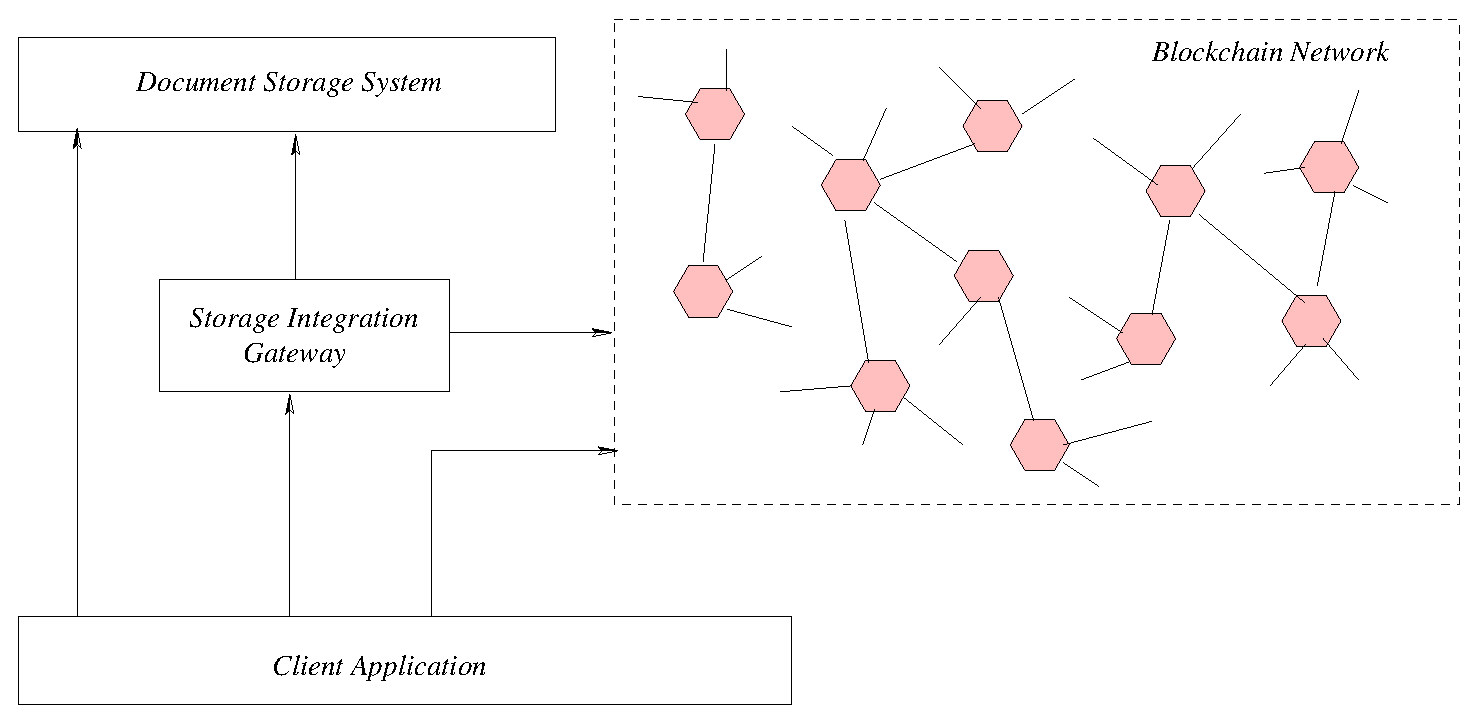
\includegraphics[width=0.48\textwidth]{system-architecture}                    
\caption{External Storage System Integration Model}\label{fig-1}
\end{figure}
Observant readers will notice that the \textit{Blockchain Network} and the back-end \textit{Document Storage} of Figure \ref{fig-1} can scale up to meet users' high-availability and other quality of service needs. However, the same cannot be said about the \textit{Gateway}. If proper care is not taken, its failure can make documents unavailable for client access. We avoided this potential problem by ensuring that the gateway database only contains information derived from the blockchain network. Hence, the gateway can be limitlessly replicated and the same back-end document storage may be interfaced by many gateways at the same time. Furthermore, we support different gateways to be configured differently to charge users for upload and/or download differently based on their quality of service (QoS) and application requirements.

The underlying core innovations that make our solution work are as follows:
\begin{enumerate}
\item Secure and accountable document upload-download protocols with flexible blockchain based payments.
\item A generic document access control configuration paradigm using blockchain smart contracts. 
\item Enforcement of access control rules in storage integration gateways.
\item Fault-tolerant design of the storage integration gateway against blockchain transaction reversal and back-end storage system failures.   
\end{enumerate}         
This paper describes these core innovations and discusses some associated concerns. The rest of the paper is organized as follows:

\subsection{Paper Organization}
Section \ref{s-scope} elaborates on the scope of the external storage integration problem in our modeling, Section \ref{s-updown} describes document upload/download protocols and analyzes their characteristics, Section \ref{s-accr} presents our innovation on blockchain smart contract based document access control policy configuration and its enforcement, Section \ref{s-gate} examines some gateway design concerns, Section \ref{s-rw} discusses some related work on blockchain based/inspired document storage, Finally, Section \ref{s-con} concludes the paper.
